\documentclass[a4paper, DIV=13]{scrartcl}

\usepackage[
typ=ib,
fach=Mathematik,
lerngruppe=2BF,
farbig,
namensfeldAnzeigen,
datumAnzeigen,
seitenzahlen = auto,
loesungen = seite,
module= {Papiertypen}
]{schule}


\usepackage{amsmath}
\usepackage{float}
\usepackage[]{fourier-otf}
\usepackage{microtype}	
\author{Maximilian Hertenstein}
\date{\today}
\title{Schnittpunkte von Geraden bestimmen}
\date{Datum: \hspace{1.5cm}}

\usepackage{tkz-base}
\usepackage{tkz-fct}
\usepackage{tkz-euclide}
\ifoot{% TODO: \usepackage{graphicx} required

		
\includegraphics[width=0.3\linewidth]{GHSE-Logo}

}

\begin{document}






\begin{minipage}{0.5\linewidth}

\begin{center}
		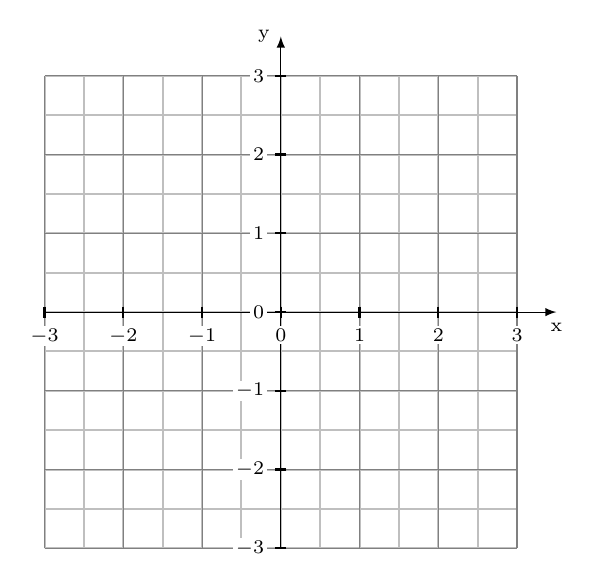
\begin{tikzpicture}[scale = 1]
			\scriptsize
			\tkzInit[ymax=3, xmax=3, xmin=-3, ymin = -3,xstep=1,ystep=1]
			\tkzGrid[sub,subxstep=0.5, subystep=0.5]
			\tkzFct[samples=50,domain=-5:5]{-x +2}
			\tkzFct[samples=50,domain=-5:5]{2*x -1}
			%\tkzSetUpAxis[line width=10pt,tickwd=0pt,ticka=0pt,tickb=0pt]
			\tkzAxeXY[/tkzdrawX/label=x,/tkzdrawY/label=y]
			
		\end{tikzpicture}

		
	\end{center}
\end{minipage}
\begin{minipage}{0.5\linewidth}

\begin{center}
		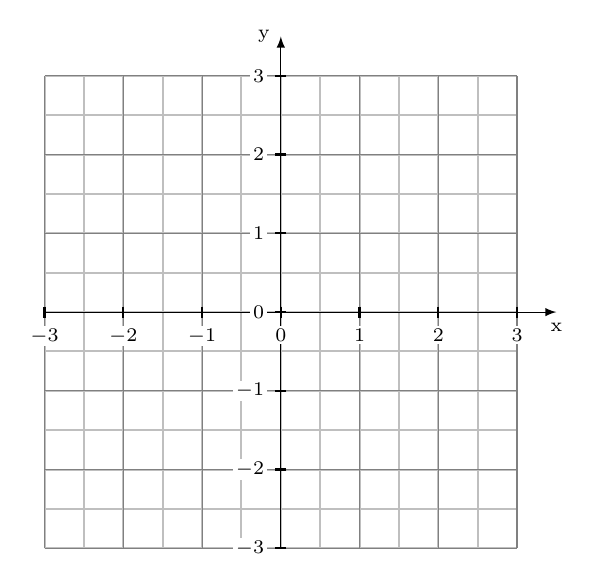
\begin{tikzpicture}[scale = 1]
			\scriptsize
			\tkzInit[ymax=3, xmax=3, xmin=-3, ymin = -3,xstep=1,ystep=1]
			\tkzGrid[sub,subxstep=0.5, subystep=0.5]
			\tkzFct[samples=50,domain=-5:5]{(-3)*x +2 }
			\tkzFct[samples=50,domain=-5:5]{(2)*x -3 }
			%\tkzSetUpAxis[line width=10pt,tickwd=0pt,ticka=0pt,tickb=0pt]
			\tkzAxeXY[/tkzdrawX/label=x,/tkzdrawY/label=y]
			
		\end{tikzpicture}

		
	\end{center}
\end{minipage}
\vskip 10pt

Der Schnittpunkt von 2 Geraden kann in einem Schaubild abgelesen werden.
\vskip 10pt

\begin{minipage}{0.5\linewidth}
$$S(\qquad, \qquad)$$


\end{minipage}
\begin{minipage}{0.5\linewidth}
$$S(\qquad, \qquad)$$

\end{minipage}

\vskip 10pt

Sie können auch aus den Wertetabellen abgelesen werden.
\vskip 10pt

\begin{minipage}{0.5\linewidth}
\begin{tabular}{|c|c|c|c|}
\hline
x & $0$ & $1$ & $2$  \\
\hline
y &\qquad & \qquad & \qquad  \\
\hline
\end{tabular}
\end{minipage}
\begin{minipage}{0.5\linewidth}
\begin{tabular}{|c|c|c|c|}
\hline
x & $0$ & $1$ & $2$  \\
\hline
y &\qquad & \qquad & \qquad  \\
\hline
\end{tabular}
\end{minipage}

\vskip 10pt

Die Schnittpunkte können auch rechnerisch bestimmt werden.


\begin{minipage}{0.5\linewidth}
\begin{align*}
f\colon y=& 2 \cdot x - 1\\
g\colon y=& -  x + 2
\end{align*}


\end{minipage}
\begin{minipage}{0.5\linewidth}
\begin{align*}
f\colon y=& 2x + 3\\
g\colon y=& -3x +2
\end{align*}

\end{minipage}

\begin{minipage}{0.5\linewidth}
\feldKar{20}
\end{minipage}
\begin{minipage}{0.5\linewidth}
\feldKar{20}
\end{minipage}


\end{document} 